%!TEX root = ../../_preamble.tex
\begin{marginfigure}[2cm]
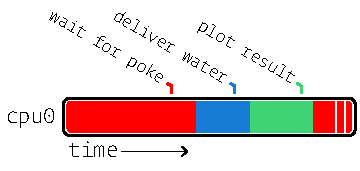
\includegraphics[]{figures/side_12_onethread.pdf}
\caption{A single-threaded program executes all operations sequentially, using a single process and cpu core.}
\label{fig:singlethread}
\end{marginfigure}

Most behavioral software is single-threaded (Figure \ref{fig:singlethread}), meaning the program will only perform a single operation at a time. If the program is busy or waiting for an input, other operations are blocked until it is finished.

Autopilot distributes computation across multiple processes and threads to take advantage of the Raspberry Pi's four CPU cores. Most operations in Autopilot are executed in \textbf{threads}. Specifically, Autopilot spawns separate threads to process messages and events, an architecture described more fully in \hyperref[sec:networking]{section \ref*{sec:networking}}. Threading does not offer true concurrency\sidenote{See David Beazley's  \href{http://www.dabeaz.com/python/UnderstandingGIL.pdf}{`Understanding the Global Interpreter Lock'} and associated \href{http://www.dabeaz.com/GIL/gilvis/index.html}{visualizations}.}, but does allow Python to distribute computational time between operations so that, for example, waiting for an event does not block the rest of the program, and events are not missed because the program is busy (Figure \ref{fig:multithread}).

\begin{marginfigure}[0.25cm]
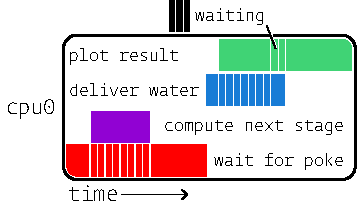
\includegraphics[]{figures/side_13_multithread.pdf}
\caption{A multi-threaded program divides computation time of a single process and cpu core across multiple operations so that, for example, waiting for input doesn't block other operations.}
\label{fig:multithread}
\end{marginfigure}

Critical operations that are computationally intensive or cannot be interrupted are given their own dedicated \textbf{processes}. Linux allows individual cores of a processor to be reserved for single processes, so individual Raspberry Pis are capable of running four truly parallel processing streams. For example, all Raspberry Pis in an Autopilot swarm create a messaging client to handle communication between devices which runs on its own processor core so no messages are missed. Similarly, if an experiment requires sound delivery, a realtime \hyperref[sec:stim]{sound engine} in a separate process (Figure \ref{fig:multiprocess}) also runs on its own core.

\begin{marginfigure}[0.1cm]
 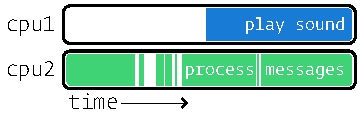
\includegraphics[]{figures/side_14_multiprocess.pdf}
 \caption{A multi-process program is truly concurrent, allowing multiple cpu cores to operate in parallel.}
 \label{fig:multiprocess}
\end{marginfigure}

Since even moderately complex experiments can consume more resources than are available on a single processor, the topmost layer of concurrency in Autopilot is to use additional \textbf{computers}. Autopilot uses the Raspberry Pi as a low-cost hardware controller, but only its GPIO control system is unique to them: the rest of the code can be used on any type of computer, so computationally expensive or GPU-intensive operations can be offloaded to any number of high performance machines. Computers divide labor \textit{autonomously} (see \ref{sec:message_handling} and \ref{sec:agents} ), so for example one computer running a task can send and receive messages from another running the GUI and plots, but does not \textit{depend} on that input as it would in a system that couples a microcontroller with a managing computer. The ability to coordinate multiple, autonomous computers with heterogeneous responsibilities and capabilities in a shared task is Autopilot's definitive design decision.